\documentclass[ngerman,aspectratio=169,10pt]{beamer}

\usetheme[progressbar=frametitle]{metropolis}
\usepackage{appendixnumberbeamer}

\graphicspath{{./graphics/}, {./../../data/scripts/runs/rules/figures/}}

\usepackage{booktabs}
\usepackage{xspace}
\usepackage{amsmath}
\usepackage{amssymb}
\usepackage{amsthm}
\usepackage{xfrac}
\usepackage{listings}
\lstset{
	basicstyle=\ttfamily,
	showstringspaces=false,
	tabsize=4,
	upquote=true,
}

\title{Labeling-Heuristiken}
% \subtitle{}
\date{09. Dezember 2020}
\author{Levin Nemesch, Joshua Sangmeister}
\institute{Algorithm Engineering - Projekt}
\titlegraphic{
    \hfill
\includegraphics[height=1.5cm]{unilogo.pdf}\\
    \hspace*{8.3cm} \textsc{AG Theoretische Informatik}
}

\begin{document}

\maketitle

\begin{frame}{SAN}
    \begin{itemize}
        \item TODO
    \end{itemize}
\end{frame}

\begin{frame}{Rules-Heuristik}
    \begin{itemize}
        \item Phase I: Anwenden der Regeln auf alle Punkte
        \item Phase II: Heuristisches Eliminieren von Kandidaten
        \vspace{10px}
        % @Levin: Falls du die Definitionen auch nutzen willst/brauchst, schieb sie gerne nach oben und schmeiß diese Folie einfach raus, die 2 Phasen kann ich auch mündlich sagen
        \item Ein \textit{Punkt} hat mehrere \textit{Kandidaten}
        \item Kandidaten können \textit{in Konflikt stehen}
        \item Die \textit{Konflikt-Partner} eines Kandidaten sind alle Kandidaten, mit denen er in Konflikt steht
        \item \textit{Konfliktzahl} eines Kandidaten: Anzahl der Konflikt-Partner
    \end{itemize}
\end{frame}

\begin{frame}{Rules-Heuristik}
    \centering
    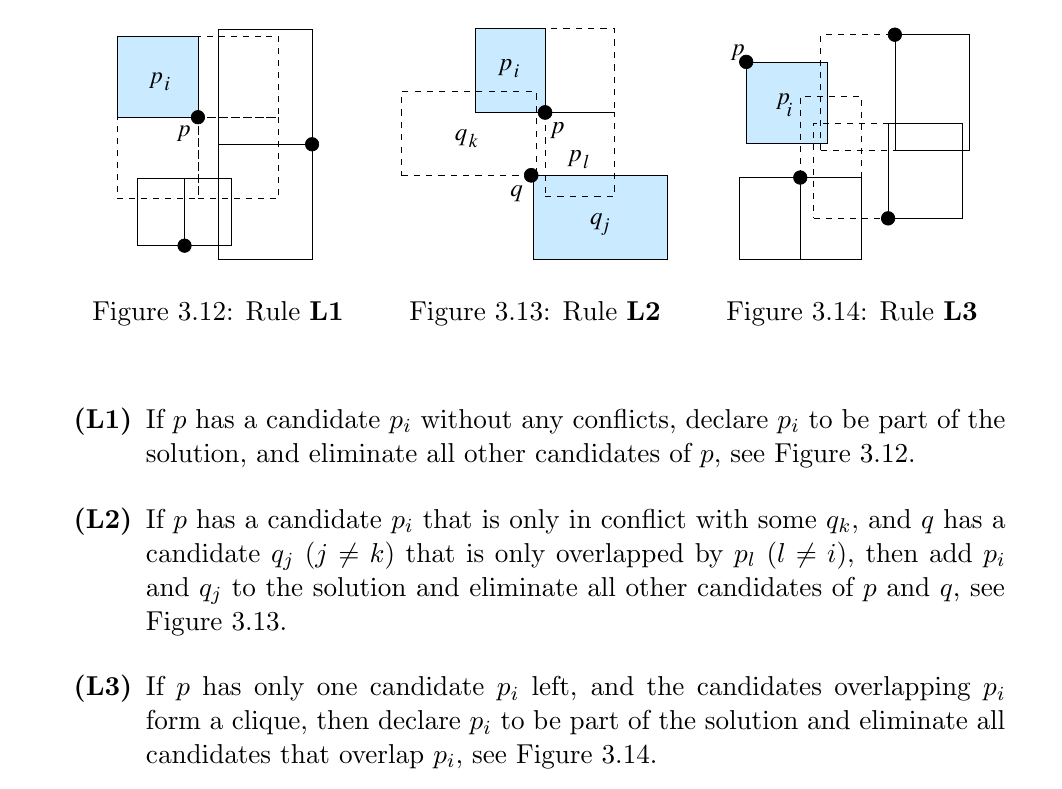
\includegraphics[width=270px]{rules}
\end{frame}

\begin{frame}{Rules-Heuristik: Ergebnisse}
    \centering
    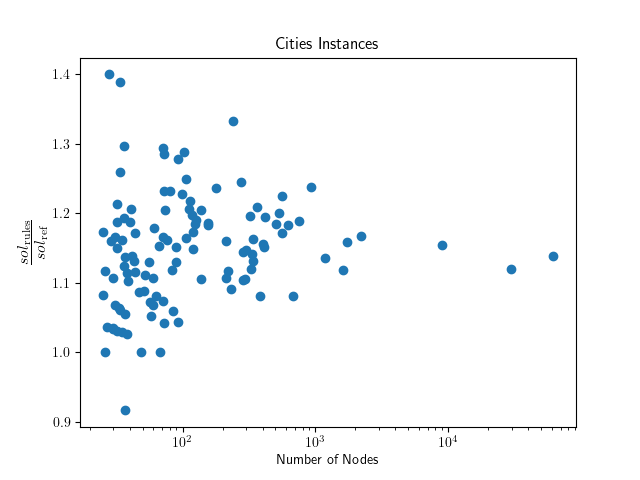
\includegraphics[width=270px]{value_rules_vs_ref}
\end{frame}

\begin{frame}{Rules-Heuristik: Laufzeit}
    \centering
    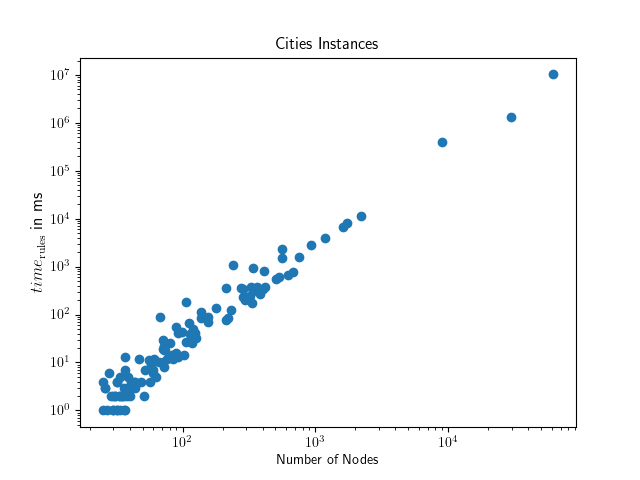
\includegraphics[width=270px]{rules_time_abs}
\end{frame}

\begin{frame}{Rules-Heuristik: Vergleich mit SAN}
    \centering
    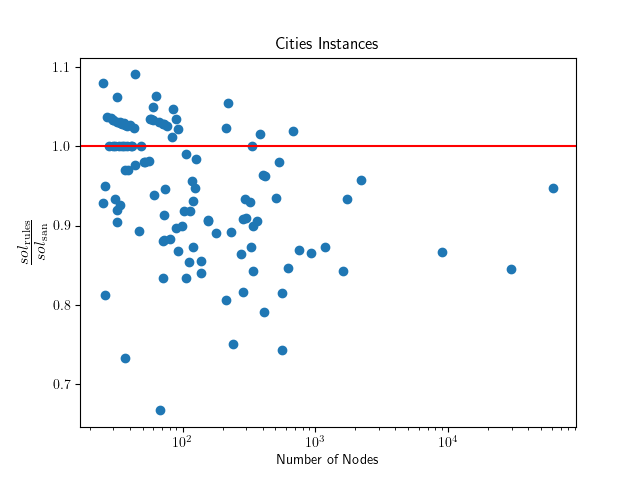
\includegraphics[width=270px]{value_rules_vs_san}
\end{frame}

\begin{frame}{Rules-Heuristik: Vergleich mit SAN: Laufzeit}
    \centering
    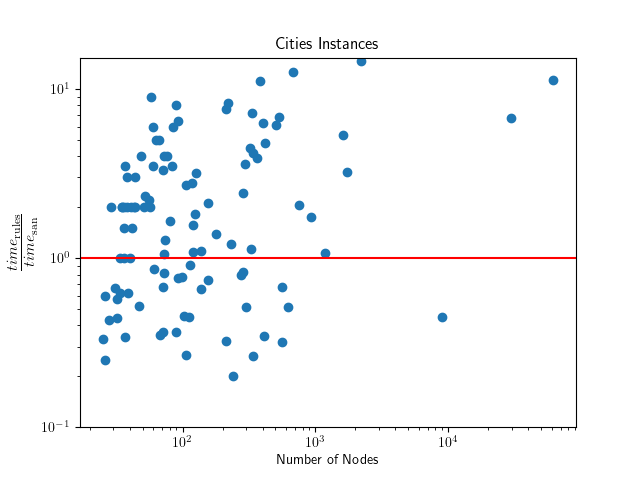
\includegraphics[width=270px]{time_rules_vs_san_1}
\end{frame}

\end{document}